\documentclass[letterpaper,12pt]{article}

\RequirePackage{comment}
\RequirePackage[hypertex]{hyperref}
\RequirePackage{GE05}
% this inputs graphicx, too

\newcommand{\NX}{\mbox{\em NX\/}}
\newcommand{\POP}{\mbox{\em POP\/}}

\def\ClassName{The Global Economy}
\def\Category{Professor David Backus}
\def\HeadName{Midterm Exam}

\begin{document}
\parindent = 0.0in
\parskip = \bigskipamount
\thispagestyle{empty}%
\Head

\centerline{\large \bf \HeadName}%
%\centerline{March 9, 2005}
\centerline{Revised:  \today}

\bigskip
You have 75 minutes to complete this exam.  Please answer each
question in the space provided. You may consult one page of notes
and a calculator, but devices capable of wireless transmission are
prohibited.


I understand that the honor code applies: I will not lie, cheat,
or steal to gain an academic advantage, or tolerate those who do.

\begin{flushright}
\rule{4in}{0.5pt} \\ (Name and Signature)
\end{flushright}


\begin{figure}[h]
    \centering
    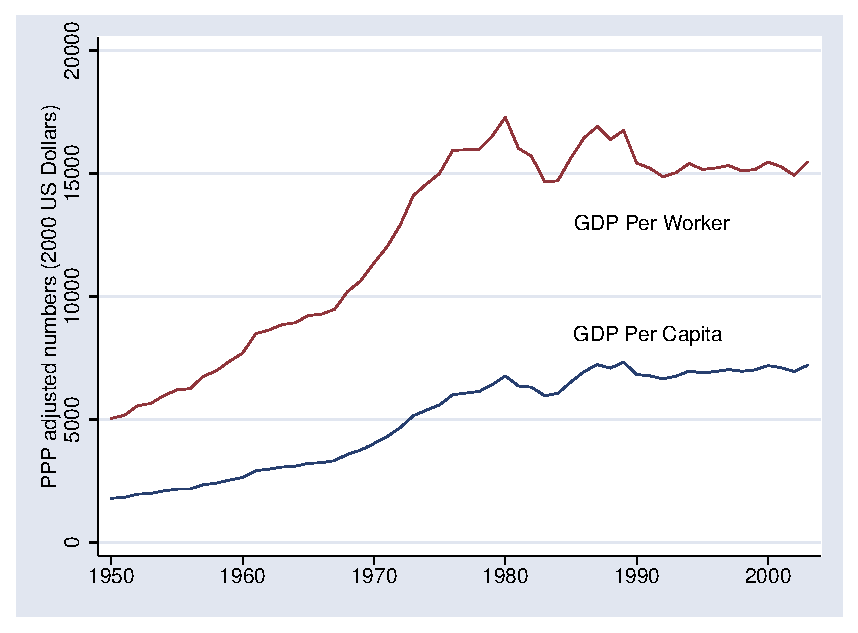
\includegraphics[scale=0.8]{pwtbramidterm07.eps}
    \caption{GDP Per Capita and GDP Per Worker in Brazil.}
    \label{fig:brazil}
\end{figure}

\begin{enumerate}
% ======================================================================
\item {\it Brazil.\/} 
As a successful European investment banker, you 
happen to have lunch with Rupert Murdoch.
Looking for a mutually beneficial topic of conversation, 
you mention the limitless opportunities of Brazil, 
which you've seen first-hand while arranging mergers 
between Brazilian and European companies.  
Murdoch calls your bluff, and asks why you see Brazil as an opportunity, 
when its recent growth experience has been modest or worse. 
You change subjects after promising to send him a short
memo the next day.  

Back in the office, 
you ask your assistant to download some Brazilian data.   
She collects the information in 
Table \ref{tab:brazil} and Figure \ref{fig:brazil}.
In the table, 
$\POP$ is population, $Y$ is real GDP, $L$ is employment 
(the number of people working), 
and $K$ is the stock of physical capital (plant and equipment).  
Population is reported in millions;
the other numbers are PPP adjusted, reported in 2000 US dollars. 
All are derived from the Penn World Tables, version 6.2.  
 
Using this data, you do a few quick calculations.
Since the figure suggests a sharp change in 1980, so 
you decide to look separately at the periods before and after 1980.
%
\begin{enumerate}

\item You compute growth rates of GDP,
GDP per capita, and GDP per worker 
for the two periods.  
What are the important differences?  
(15~points)

\item Since GDP per capita and GDP per worker are similar, 
you decide to focus on the latter and 
decompose its growth in each period into components
due to capital per worker and total factor productivity.  
Which component accounts for the difference between 
the two periods?  
(15~points)

\item You are looking for a positive tone to your memo.
What exactly can you claim is growing in Brazil?  (10~points)

\end{enumerate}


\begin{table}
    \centering 
    \tabcolsep = 0.2in
    \begin{tabular}{lcccc}
    \hline\hline
    Year    &  $ \POP $   &  $Y/\POP$   &  $Y/L$  &  $K/L$  \\
    \hline\hline
    1950 & \phantom{1}53,443  &   1,802  &  5,045   &  \phantom{1}8,559  \\
    1980 &   122,958  &   6,776  &  17,285\phantom{1}  & 39,064  \\
    2003 &   182,033  &   7,205  & 15,462\phantom{1} & 37,604    \\
    \hline\hline
    \end{tabular}
    \caption{Aggregate Data for Brazil.}
    \label{tab:brazil}    
\end{table}

%\begin{comment}
Answer.
\begin{enumerate}

\item We compute continuously-compounded growth rates the usual way.
The results are summarized in Table \ref{tab:brazil-growth}.
With both measures, growth effectively halted in 1980.  

\item The usual growth accounting exercise.  
First we compute TFP ($A$):  
247 in 1950, 509 in 1980, and 462 in 2003.
Apparently TFP growth has disappeared.  
The growth rates of the various components are listed 
in Table \ref{tab:brazil-growth}.
Our decomposition of the growth rate of output per worker is 
\[
        \gamma_{Y/L} \;=\; \gamma_A + \alpha \gamma_{K/L}  
\]
with $\alpha = 1/3$.  
For the two periods, we get 
\begin{eqnarray*}
    \mbox{1950-1980:} &&  4.1  \;=\; 2.4 \mbox{ (A)} +  1.7 \mbox{ (K/L)}   \\
    \mbox{1980-2003:} &&  -0.5 \;=\; -0.4 \mbox{ (A)} -  0.1 \mbox{ (K/L)} .
\end{eqnarray*}

\begin{table}
    \centering 
    \tabcolsep = 0.2in
    \begin{tabular}{lcccc}
    \hline\hline
    Period    &   $Y/\POP$   &  $Y/L$  &  $K/L$  &  $A$ \\
    \hline\hline
    1950-1980 &  4.4 &  4.1  &  5.1   & 2.4  \\
    1980-2003 &  0.3 & (0.5) &  (0.2) & (0.4)  \\
    \hline\hline
    \end{tabular}
    \caption{Various growth rates for Brazil (percent).}
    \label{tab:brazil-growth}    
\end{table}


\item Although GDP per capita and GDP per worker are not growing, 
GDP is, since there are more people, and more people working.
The growth rate of GDP itself was 7.0\% in the first period, 
2.0\% in the second.
You have no way of knowing this, but there's also a difference 
between the PPP-adjusted numbers reported in the Penn World Tables
and Brazil's official ``real GDP'' data.
Which you trust more is hard to say. 
Despite all this, it's hard to avoid concern about the Brazilian 
economy.  

\end{enumerate}
%\end{comment}


\pagebreak \phantom{xx} \pagebreak \phantom{xx} \pagebreak
% ======================================================================
\item {\it Vietnam.\/} 
Since 1991, Vietnam's per capita GDP has
been growing at an average rate of 6.75\%, positioning the
Southeast Asian economy among the fastest growing in the world. 
According to analysts, an obstacle to even speedier
growth will likely be removed shortly when Vietnam 
joins the World Trade Organization.

Some facts.  
In 2005, manufacturing and construction accounted for 41\% of GDP (up
from 38\% in 2001) and services for 38\% (from 27\%), whereas agriculture dropped to 21\% (from 23\%).
Employment is divided among the three sectors in the following
proportions: 17\%, 25\%, and 57\%, respectively (the service figure
includes 10\% in state employment). Female labor force participation
is high by world standards, with women accounting for 49\% of the
labor force. According to the World Bank, school enrollment rates
are 100\% in primary school, 70\% in secondary school, and 10\% in
university.  

The most notable immediate effect of
WTO membership will be the scrapping of US quotas on garment imports
from Vietnam. While these quotas limit Vietnamese exports to the
US, some analysts warn that their removal may have a relatively
modest effect: the EU's decision to waive its import quotas this year 
had only a small effect on shipments, probably because of strong
competition from other producers, particularly China. 
A further difficulty is the spate of strikes in foreign-owned factories, 
which led the government to raise the minimum wage paid by foreign firms
by 40\%.  See the attached article in {\it The Economist\/}.  

\begin{enumerate}

\item 
In which broad sectors is Vietnam likely to shift its
production in the next five years?  20 years?  
Why? (10~points)

\item To comply with the conditions for WTO membership, the
Vietnamese National Assembly recently passed two pieces of
legislation that may have a substantial impact on the
economy. The Anti-corruption Law, which comes into effect June
1st, is intended to improve the detection and prevention of public
official corruption.  The Law on Investment, also
expected to come into effect in mid-2006, allows investment projects worth
less than \$1m to proceed without registration, and projects
valued at less than \$19m  will need to be registered but will not
require licenses.   

Describe --- concretely --- how each of these changes are likely to effect 
the economy's total factor productivity.
(10~points)

\item In your view, what government policies are likely to be 
most effective in raising the living standard of the Vietnamese people 
over the next 25 years?  Why? (10~points)

\end{enumerate}

\begin{comment}
Answer.  
\begin{enumerate}
\item 
In recent times, agriculture has fallen as a fraction of GDP, 
and the other two sectors have increased their shares.  
We'd expect that to continue for two reasons.
One is that this is a standard pattern for developing countries, 
including the US 150 years ago:  people move off farms.  
Another is that this reflects the (admittedly crude) productivities 
implied by the GDP and employment shares:  
17\% of the workforce produces 41\% of GDP in manufacturing 
and construction, 
whereas 57\% of the workforce produces only 21\% of GDP in agriculture.  
Some of this might reflect differences in skill level 
and capital per worker across industries, but it's likely that 
productivity is lower in agriculture, 
and that market forces will reallocate people from agriculture 
into manufacturing --- and maybe services, too.    

\item Each of these changes should reduce the cost of running a business, 
which will increase TFP directly.
The investment law, in particular, 
should make it easier to start new businesses,  
which should facilitate the reallocation described above. 
As the economy shifts resources to more productive sectors, 
overall TFP will increase.  
It's the same argument we used with international trade.   


\item There are lots of sensible answers.  
We'd stress flexible labor markets; 
competitive product markets, including competition from abroad; 
and a legal system that enforces property rights.  

\end{enumerate}
\end{comment}


\pagebreak \phantom{xx} \pagebreak \phantom{xx} \pagebreak
% ======================================================================
\item {\it Miscellany.\/}
\begin{enumerate}

\item {\it Bridge to nowhere.\/}
In the context of our production function, would 
the construction of an economically useless bridge in Alaska lead 
(once it's completed) 
to a change in total factor productivity?  
Please explain your answer.  (10~points) 

\item {\it Labor markets and trade.\/}
An analyst at the OECD commented that the difficulty Italy has had 
adapting to increasing international trade 
was a reflection of its rigid labor markets, 
which discourage Italian businesses from the restructuring needed to 
compete in global markets.
Do you find this argument persuasive?   Why or why not?  (10~points)

\item {\it Off-shoring.\/} 
The term \textit{off-shoring} refers to 
the relocation of work from one country (the US, say) to another
(India, for example).  
Greg Mankiw, Bush's former economic advisor, suggested that 
such trade in labor services was no different than 
trade in goods:  the goal remains for countries 
to perform those tasks it does relatively efficiently.
Do you agree?  Why or why not? 
Would your answer change if you viewed the issue from the 
perspective of the in-shoring country?  (10~points)
\end{enumerate}

\begin{comment}
Answer.  
\begin{enumerate}

\item TFP falls.  The production function is 
\[
    Y \;=\; A K^\alpha L^{1-\alpha} .
\]
A new bridge increases the capital stock $K$.
If it leads to no additional output (it's ``useless'') then 
$A$ must fall.  

\item Sounds right to me.  
Rigid labor markets make it difficult for 
the Italian economy to shift people from 
their current low-productivity jobs to 
others.  

\item Almost all economists, even liberal ones, 
would agree with Mankiw:
have people do the jobs at which they are relatively most
productive.  
In the long run, that produces a higher standard of living.
That's as true for one country as it is for the other.  
Of course, individuals may be concerned with the disruption that might 
generate in their own lives, 
but there's little question where the greater good lies.   

\end{enumerate}
\end{comment}

\end{enumerate}

\pagebreak \phantom{xx} \pagebreak \phantom{xx} 
%\end{document}
\newpage
Trouble at the mill \\
Jan 26th 2006 |  HANOI \\
From The Economist print edition 

Strikes and pay rises afflict the new South-East Asian tiger

FACTORY workers in Vietnam have an extra reason to celebrate Tet, the lunar new year holiday that begins this weekend. Their government recently decided to raise the minimum wage in foreign-owned factories by up to 40\%, starting on February 1st. Pay packets in Hanoi and Ho Chi Minh City will now start at \$45 a month, the first mandated rise in several years. Experienced workers can expect an extra 7\% increase on top of that.

What is especially unsettling for investors is how the workers got their extra dough. Since late December, wildcat strikes have swept through the industrial zones surrounding Ho Chi Minh City. Tens of thousands of workers joined the protests over wages and conditions. Some of these turned violent, and machines were wrecked at one Taiwanese-owned plant. Bosses claim that outside agitators stoked the protests, distributing notes at factory gates while police stood idly by.

Apparently caught off-guard, the government issued a decree earlier this month raising the minimum wage in foreign-owned factories. Most strikers have now returned to work, but some have not, and investors are fuming over production stoppages and a higher wage bill. The European Chamber of Commerce has gone so far as to write a tart letter to the prime minister, Phan Van Khai, reminding him that investors set up shop in Vietnam precisely because ``the workforce is not prone to industrial action.''

At least, not until now. Workers in Vietnam have staged walkouts before, particularly over alleged mistreatment by foreign managers, but the scale and co-ordinated nature of the latest strikes are, well, striking. Some observers find it implausible that they could occur without the prior knowledge of the ruling party, which forbids independent trade unions. As in China, workers are allowed to join only a pliant, party-affiliated union.

Most of the affected factories are owned by East Asian companies, the biggest investors in Vietnam. At Song Than industrial zone, on the outskirts of Ho Chi Minh City, 80\% of the factories are owned by Taiwanese, producing clothing, shoes, furniture and bicycles for export. They grumble that higher wages will drive away foreign investment, running at \$5.8 billion last year, and give warning that Vietnam needs to stay competitive. ``Chinese wages are higher. But the quality and efficiency are also higher,� said Chen Chi Young, an official at Taiwan's de facto embassy.

So why didn't Vietnam crush the illegal strikes? One reason, say observers, may be internal jockeying ahead of the party congress in April, a five-yearly affair. The aim could have been to embarrass the provincial officials where the unrest began, or to burnish the leadership's credentials, or both. The factories most affected may also be a clue: Vietnam and Taiwan both claim ownership of the Spratly Islands, along with several other countries. On December 15th, Taiwan said it was building a landing strip on one of the islands.

Or perhaps the workers were simply fed up with low pay and stingy bosses, and were too numerous to repress. Vietnam has one of the world's fastest growing economies. Now it is learning that higher output means higher expectations.


\end{document} 